\chapter{Background}
\label{chap:background}
\graphicspath{{Chapter3/Figs/}}

\begin{chapabstract}
Firstly, chapter \ref{chap:background} presents the theoretical background used in the thesis including malware types, PE file format and academic background in machine learning. Then, machine learning frameworks and tools are introduced to reveal our implementation in practice.
\end{chapabstract}

\section{Malware Types}
\label{sec:malware}

Classifying is the excellent way to have a better understanding of malware. There are several of the most common types: adware, bots, rootkits, spyware, Trojan horses, viruses, and worms \cite{neil2012common}.

\subsection{Virus}

A virus is a form of malware that is capable of replicating itself and spreading to other computers by attaching themselves to various applications and executing when a user launches one of those. Viruses can also spread through documents, script files, and cross-site scripting vulnerabilities in web apps. Some famous examples of viruses over the years are the Concept virus, the Chernobyl virus (also known as CIH), the Anna Kournikova virus, Brain, and RavMonE.exe.

\subsection{Worm}

A worm is a standalone software that replicates without targeting and infecting specific files. Think of worms as small programs that replicate themselves and destroy the data. They usually aim the operating system files and work until the drive they are in becomes empty. Some examples include Melissa, Morris, Mydoom, Sasser, and Blaster.

\subsection{Trojan}

A Trojan is a malicious application that misrepresents itself to look useful to fool users into downloading and installing. A trojan can give remote access to an infected computer which is possible for the attacker to steal data, install more malware, monitor user activity, etc. Notable examples also include Trojan horses developed by United States government agencies like the FBI and NSA. Names like Magic Lantern, FinFisher, Netbus, Beast, Gh0st RAT, Clickbot.A, and Zeus have been the reason of horror. While an Android malware discovered in 2015, called Shedun, is one of the many that target mobile devices.

\subsection{Ransomware}

Ransomware, which is one of the most advanced and continuously on the rise these days, is a kind of malware that typically holds a computer system captive while requiring a ransom, e.g., blocking the access to the data of a victim or threating to either publish it. Worse yet, there is no guarantee that paying will get access to the data, or prevent it from publishing. Major ransomware like Reveton, CryptoLocker, CryptoWall, and more recently, the 2017 WannaCry attack, have caused no small amount of destruction \cite{chen2017automated}.

\subsection{Rootkit}

A rootkit is a collection of software specially designed to allow malware that gathers information, into your system. These work in the background so that a user may not notice anything different. But in the environment, a rootkit will permit several types of malware to get into the system. The first rootkit to gain reputation on Windows was NTRootkit in 1999, but the most popular is the Sony BMG copy protection rootkit scandal that shook the company in the year 2005 \cite{bruce2005sony}.

\subsection{Adware}

Although the advertising-supported software (adware) is now much more common and known as adware in some circles, this word has been linked to malware for quite some time. While adware can refer to any application that is supported by advertising, malicious adware usually displays ads in the form of popups and windows that cannot be closed. It is the perhaps the most productive and least dangerous malware, designed with the specific purpose of promoting ads on your computer.

\subsection{Bot}

Bots are software programs created to perform specific operations automatically. While some bots are created for approximately innocent purposes, it is becoming increasingly common to see bots being used maliciously. Bots can be used in botnets (collections of machines to be controlled by third parties) to perform distributed denial of service attacks, send spam, and steal data.

\section{PE File Format}
\label{sec:pe-file}

The Portable Executable (PE) file format describes the predominant executable format for Microsoft Windows operating systems and includes executables, dynamically-linked libraries (DLLs), and FON font files. The format is currently supported on Intel, AMD, and variants of ARM instruction set architectures.

A Portable Executable file consists of some headers and sections that tell the dynamic linker how to map the file into memory. An executable image includes of several different regions, each of which requires different memory protection; so the start of each section must be aligned to a page frame. Typically, headers include the Common Object File Format (COFF) file header that contains essential information such as the type of machine for which the file is intended, the nature of the file (DLL, EXE, OBJ), the number of sections, the number of symbols, etc. The optional header identifies the linker version, the size of the code, the size of initialized and uninitialized data, the address of the entry point, etc. Data directories within the optional header provide pointers to the sections that follow it. These sections include tables for exports, imports, resources, exceptions, debug information, certificate information, and relocation tables. So, it provides a useful summary of the contents of an executable \cite{shafiq2009pe}. Finally, the section table outlines the name, offset and size of each section in the PE file.

\begin{figure}[H] 
\centering    
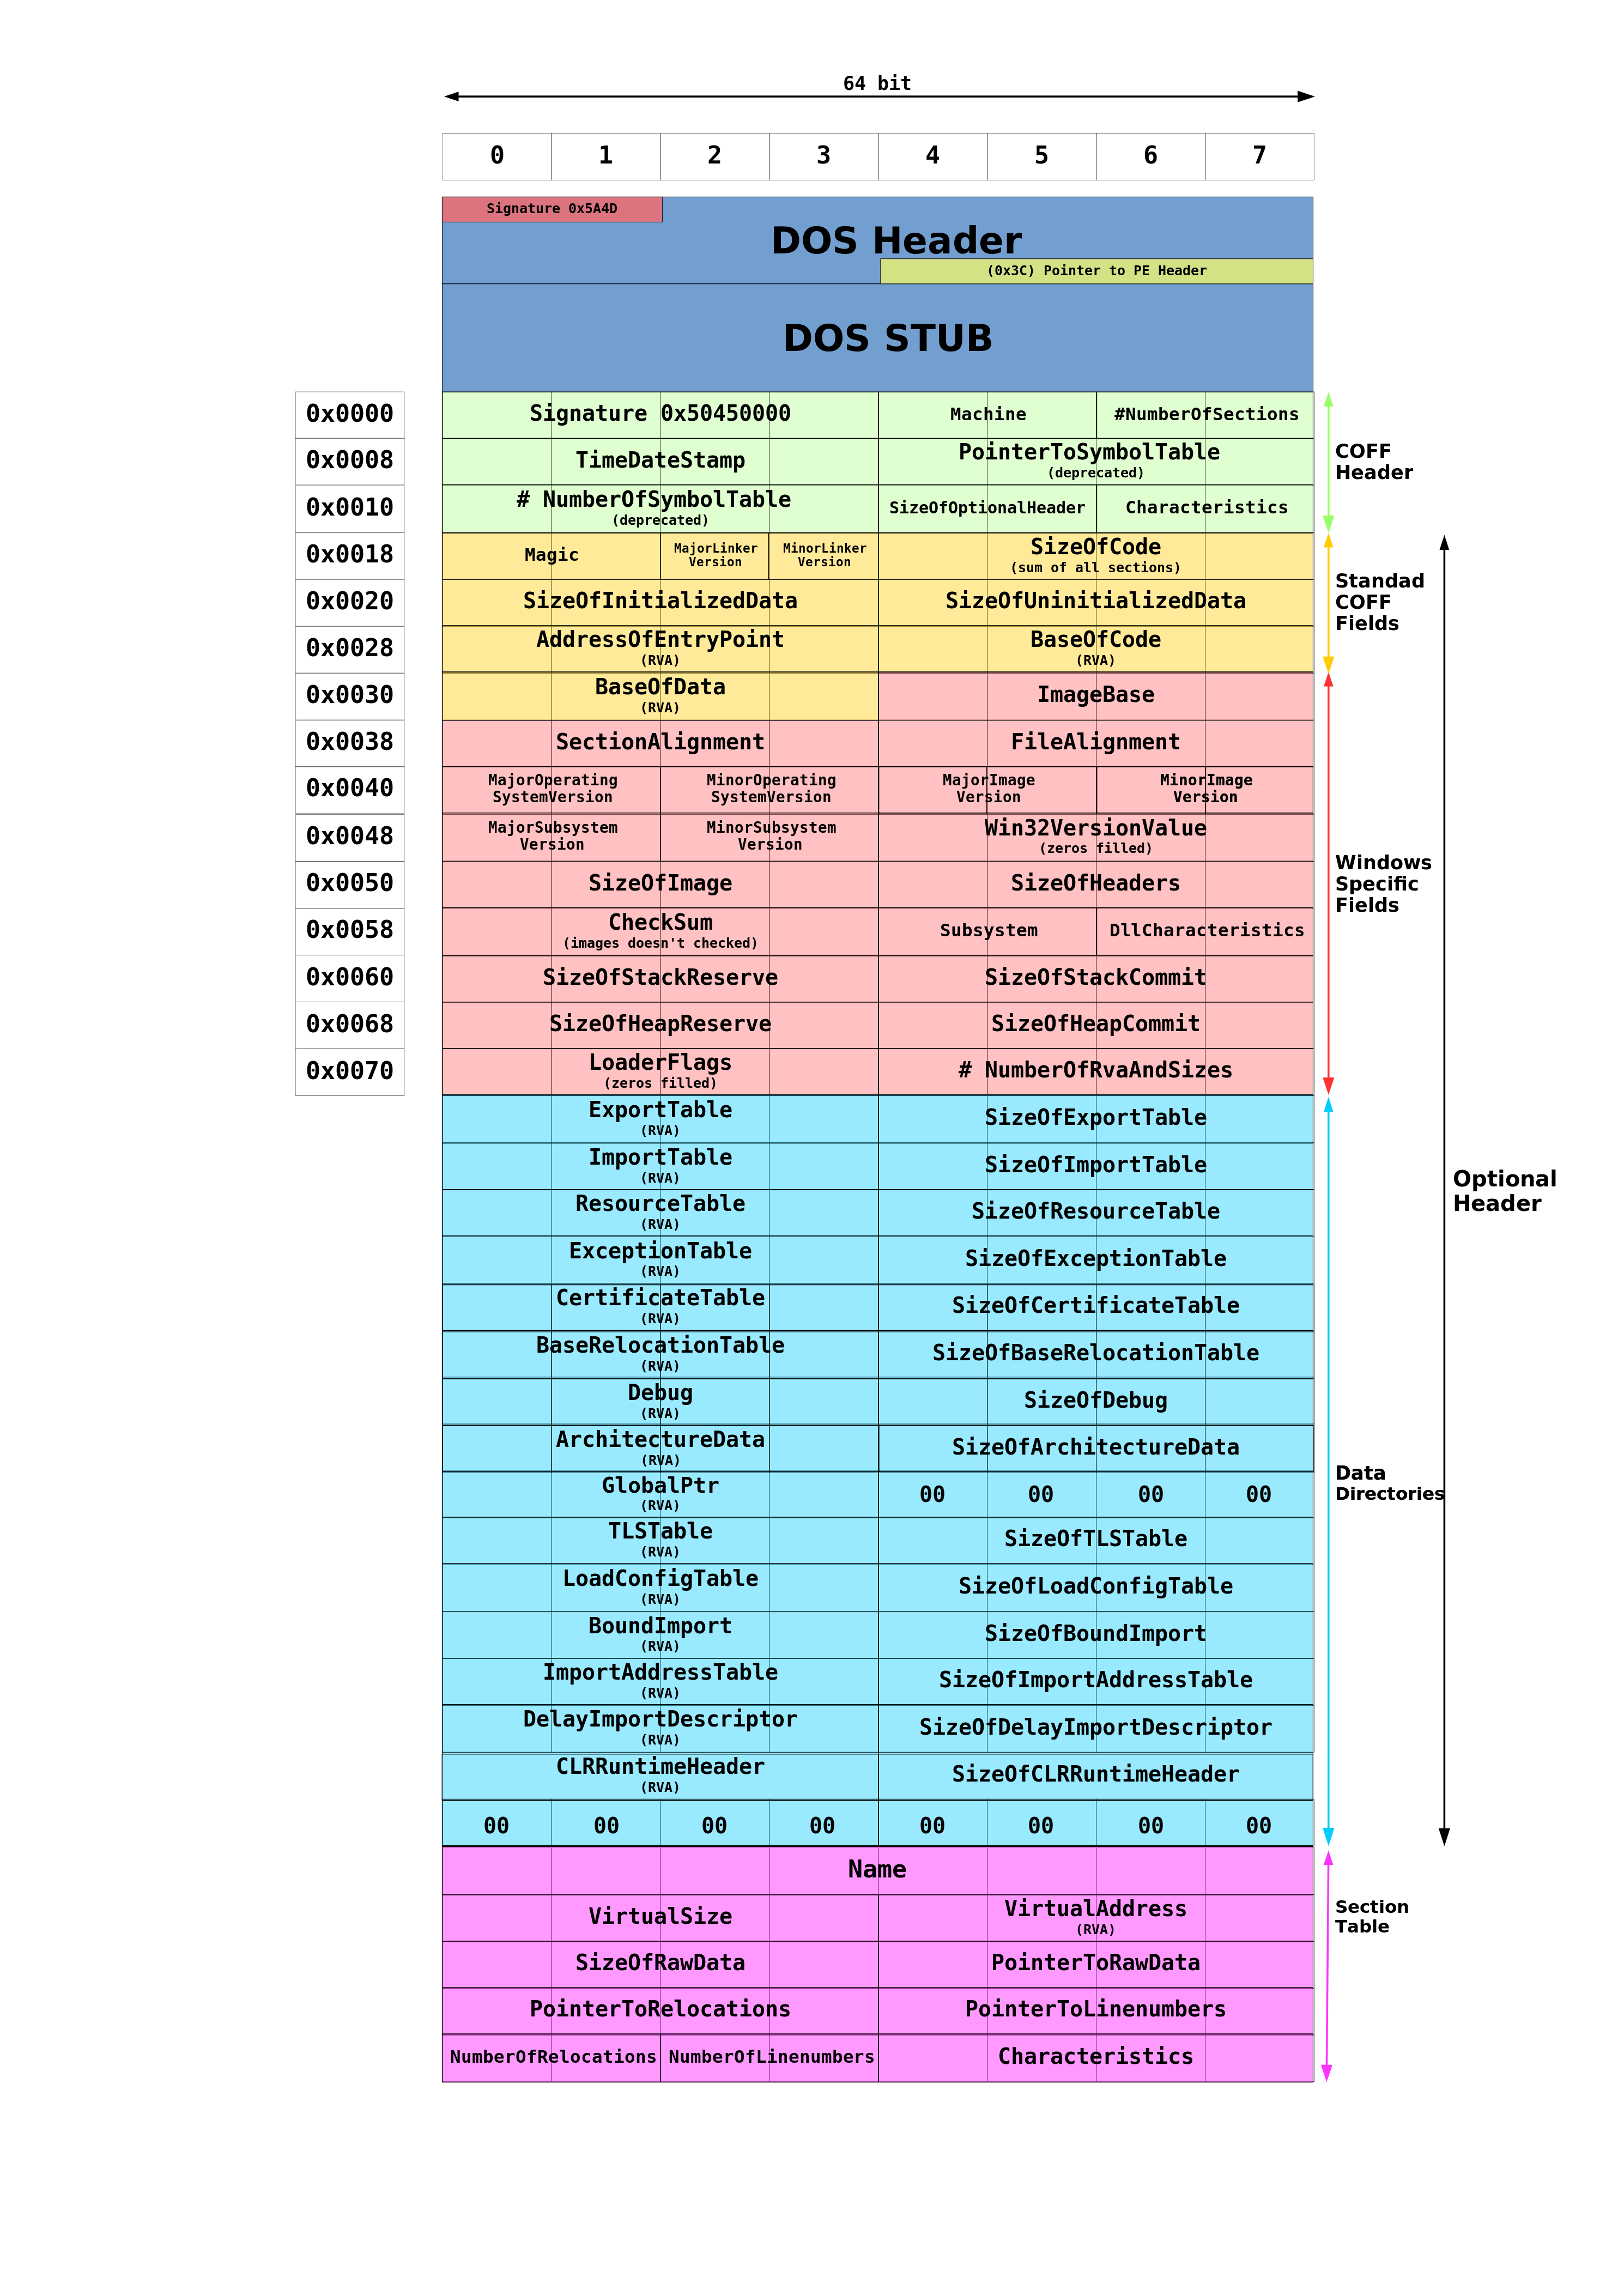
\includegraphics[width=1.0\textwidth]{Portable_Executable_32_bit.png}
\caption{Structure of a Portable Executable 32 bit \cite{wikipefile}}
\label{fig:pe32bit}
\end{figure}

PE sections contain code and initialized data that the Windows loader is to map into executable or readable/writeable memory pages, individually, as well as imports, exports, and resources defined by the file. Each section contains a header that specifies the size and address. An import address table instructs the loader which functions to import statically. A resources section may contain resources required for user interfaces such as: cursors, fonts, bitmaps, icons, menus, etc. A basic PE file would commonly contain a .text code section and one or more data sections (.data, .rdata or .bss). Relocation tables are typically stored in a .reloc section, used by the Windows loader to reassign a base address from the executable’s preferred base. A .tls section contains special thread local storage (TLS) structure for storing thread-specific local variables. Section names are random from the perspective of the Windows loader, but specific names have been adopted by precedent and are overwhelmingly common.

\section{Machine Learning}

\subsection{Introduction}
\label{ssec:machine-learning-intro}

In recent years, most of the productive research and advancements have come from the sub-discipline of Artificial Intelligence named Machine Learning. The principle of Machine Learning is straightforward; Machine Learning is a method by which computers find patterns in data and makes those patterns available to applications. The application can then gain insights on new data based on similarity to the identified patterns \cite{martin2016machine}.

\begin{figure}[htbp!] 
\centering    
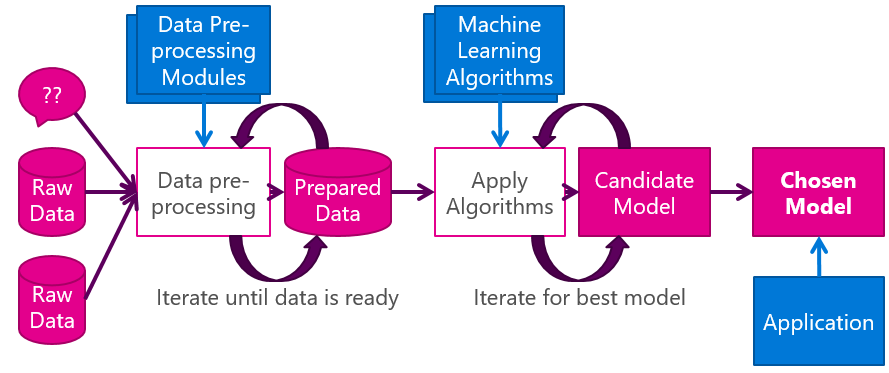
\includegraphics[width=1.0\textwidth]{MLProcess.png}
\caption{Machine Learning process \cite{martin2016machine}}
\label{fig:ml-process}
\end{figure}

It is worth going through the general workflow (Figure \ref{fig:ml-process}) of the machine learning process to have a deeper understanding:

\begin{itemize}
\item The primary goal of the process is to identify a model. The model is the main thing that applications can submit requests to gain insight on new data.
\item Before moving into Machine Learning experiments, we must identify the purpose and how to evaluate the result.
\item The process starts with preparing data. Prepared data is one or more data sets that have been preprocessed (formatted, cleaned and sampled) in readiness to apply Machine Learning algorithms. Preparing the data means that the data is in the best shape to draw scientific conclusions.
\item The next step is applying one or more Machine Learning algorithms intending to producing a Model, which is an iterative process and we may loop around testing various algorithms until we achieve a model that sufficiently reach the purpose.
\end{itemize}

Not all problems are candidates for a machine learning solution. The problem must be one that can be solved with data, and a sufficient quantity of relevant data must exist and be acquirable. As we shall see, many security problems fit this profile exceedingly well.

\subsection{Supervised Learning}
\label{ssec:supervised-learning}

Supervised learning algorithms make predictions based on a set of samples, e.g., historical stock prices can be used to try to guess at future prices. A supervised learning algorithm looks for patterns in labeled data. It can use any information that might be relevant, and each algorithm looks for different types of patterns. After the algorithm has detected the best pattern it can, it uses that pattern to make predictions for unlabeled data.

When the data are being used to predict a category, supervised learning is also called classification, e.g., assigning an image as a picture of either a cat or a dog. When there are only two choices, it is called two-class, binomial or binary classification. When there are more categories, this problem is known as multi-class classification.

\subsection{Feature Extraction}

As mentioned in section \ref{ssec:machine-learning-intro}, we should extract the attributes from the input data so that we can feed it into the algorithm. For example, in the image cases, data can be represented as an RGB value of each pixel.

Such attributes are referred to \textbf{features}, and the matrix is referred to as feature vector. The process of extracting data from the files is called feature extraction. The goal of feature extraction is to obtain a set of informative and non-redundant data. 

It is essential to understand that features should represent the necessary and relevant information about our dataset since we cannot make an accurate prediction without it. That is why feature extraction is often a non-obvious and domain-specific task, which requires a lot of testing and research.

Another critical requirement for a suitable feature set is non-redundancy. Having redundant features, i.e., elements that outline the same information, as well as irrelevant information attributes, that are strictly dependent on each other, can make the algorithm biased and, accordingly, provide an inaccurate result.

Furthermore, if the input data has too many features, it will take more training time. Hence, we may need to reduce the vector dimensions, which is known as the feature selection.

\subsection{Classification, Regression and Thresholding}

\textbf{Classification} is the task of approximating a mapping function ($f$) from input variables ($X$) to discrete output variables ($y$). The output variables are often called labels or categories. The mapping function predicts the class or group for a given observation. For example, an email can be classified as belonging to one of two categories: "spam" and "not spam".

\textbf{Regression} is the task of approximating a mapping function ($f$) from input variables ($X$) to a continuous output variable ($y$). An output variable is a real-value, such as an integer or floating point value. These are often quantities, such as amounts and sizes. For example, a house may be predicted to sell for a specific dollar value, perhaps in the range of \$100,000 to \$200,000.

Classification problems are different from regression problems. Classification is the task of predicting a discrete class label, and regression is the task of predicting a continuous quantity. However, there is some overlap between the algorithms for classification and regression.
For example, we can use the probability, which is returned from logistic regression, "as is" or convert it to a binary value. To map a logistic regression value to a binary category, we must define a \textbf{classification threshold} (also called the decision threshold). It is tempting to assume that the classification threshold should always be 0.5, but thresholds are dependent on the specific problems, and therefore values that we must tune.

\subsection{Ensemble, Bagging and Boosting}

When we try to predict the target variable using any machine learning method, the leading causes of difference in original and predicted values are noise, variance, and bias. The ensemble helps to reduce these two last factors.

An ensemble is just a collection of predictors which come together (e.g., mean of all predictions) to give a final prediction. The principal reason is that many different predictors trying to predict same target variable will perform a better job than any single one alone. Ensembling techniques are further classified into Bagging and Boosting.

Bagging is a simple ensembling technique in which we build many independent models and combine them using some model averaging methods (e.g., weighted average, majority vote or normal average). We typically use random sub-sample of data for each model, so that all the models are little different from each other. Each observation has the same probability to appear in all the models. Because this technique takes many uncorrelated predictors to make a final model, it reduces error by reducing variance. One example of bagging ensemble is Random Forest (which is mentioned in section \ref{ssec:random-forest}).

Boosting is an ensemble technique in which the models are not made sequentially. This technique applies the logic in which the following predictors learn from the mistakes of the previous ones. Accordingly, the observations have an unequal probability of appearing in subsequent models. The predictors can be chosen from a range of models like decision trees, regressors, classifiers, etc. Because new predictors are learning from mistakes committed by previous predictors, it takes fewer iterations to reach close to actual predictions. But we have to choose the stopping rules carefully, or it could lead to overfitting on training data. Gradient Boosting Decision Tree, in section \ref{ssec:gbdt}, is an example of boosting algorithm.

\section{Machine Learning Methods}

\subsection{Decision Tree}
\label{ssec:decision-tree}

As it assumes from the name, decision trees are data structures that have a structure of the tree. The training dataset is used for the creation of the tree, that is consequently used for making predictions on the test data. In this algorithm, the goal is to achieve the most accurate result with the least number of the decisions that must be made. We can use decision trees can for both classification and regression problems. There is an example in Table \ref{table:decision-tree}.

\begin{table}[h]
\caption{An example of decision tree}
\centering
\label{table:decision-tree}
\begin{tabular}{c l l c c c c}
\hline
Id & Name                       & Sex    & Age  & SibSp & Survived \\	
\hline
1  & Braund, Mr. Owen Harris    & male   & 22.0	& 1     & 0	\\
2  & Cumings, Mrs. John Bradley & female & 38.0	& 1     & 1	\\
3  & Heikkinen, Miss. Laina	    & female & 26.0	& 0     & 1 \\
...& ...                        & ...    & ...  & ...   & ... \\ 
\hline 
\end{tabular}
\end{table}

\begin{figure}[htbp!] 
\centering    
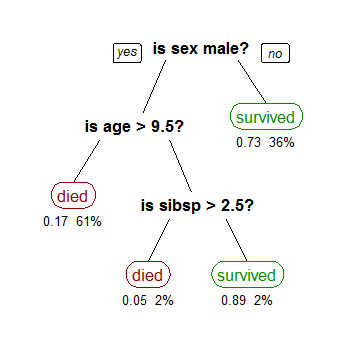
\includegraphics[width=0.5\textwidth]{decision_tree.png}
\caption{An example of decision tree \cite{wikidecisiontree}}
\label{fig:decision-tree}
\end{figure}

As you can see in Figure \ref{fig:decision-tree}, the model was trained based on the dataset and can now classify the passenger in Titanic is survived or not. The tree consists of the decision nodes and leaf nodes, and decision nodes may have several branches leading to leaf nodes. Leaf nodes represent the decisions or classifications. The first initial node is referred to as root node.

Decision tree method gained its popularity because of its simplicity. It can deal well with large datasets and can handle the noise in the datasets very well. Another advantage is that unlike other algorithms, such as SVM or KNN, decision trees operate in a white box, meaning that we can see how the outcome is obtained and which decisions led to it.

\subsection{Random Forest}
\label{ssec:random-forest}

Random Forest is one of the most common machine learning algorithms. It requires almost no data preparation and modeling but usually ends in inaccurate results. Random Forests are based on the decision trees described in the previous section \ref{ssec:decision-tree}. More specifically, Random Forests are the collections of decision trees, producing a better prediction accuracy. That is why it is called a forest – it is a set of decision trees.

The essential idea is to grow multiple decision trees based on the independent subsets of the dataset. At each node, \textit{n variables} out of the feature set are selected randomly, and the best split on these variables is found.


We can describe the algorithm as follows \cite{biau2012analysis}:

\begin{enumerate}
\item Multiple trees are built approximately on the two third of the training data randomly.
\item Several variables are randomly selected out of all the predictor variables. Then, the best split on these is used to split the node. By default, the amount of the selected variables is the square root of the total number of all predictors, and it is constant for all trees.
\item With the rest of the data, the misclassification rate is calculated. The total error rate is calculated as the overall out-of-bag error rate.
\item Each trained tree gives its classification result and the class that received the highest score is chosen as the result.
\end{enumerate}

Since we are using multiple decision trees, this algorithm removes the need for feature selection for removing unnecessary features – they will not be taken into account in any case. The only need for any feature selection with the random forest algorithms arises when there is a demand for dimensionality reduction. Moreover, the out-of-bag error rate, which was mentioned earlier can be considered the algorithm’s cross-validation method. This removes the need for tedious cross-validation measures, that would have to be taken otherwise \cite{mitchell1997machine}.

Random forests inherit many of the advantages of the decision trees algorithms. They are suitable for both regression and classification problems; they are easy to compute and quick to fit. They also regularly result in the better accuracy. However, unlike decision trees, it is not very easy to interpret the results. In decision trees, by examining the resulting tree, we can gain valuable information about which variables are relevant and how they affect the result. Random forests can also be described as a more firm algorithm than the decision trees since it is the combination of many decision trees, the random forest will remain stable \cite{louppe2014understanding}.

\subsection{Gradient Boosting Decision Trees}
\label{ssec:gbdt}

Gradient Boosting Decision Tree (GDBT) is an ensemble model of decision trees, which are trained in sequence \cite{friedman2001greedy}. 
In each iteration, GBDT learns the decision trees by fitting the negative gradients (also known as residual errors).
The main cost in GBDT lies in learning the decision trees, and the most time-consuming part of learning a decision tree is to find the best split points.
One of the most common algorithms to find split points is the pre-sorted algorithm \cite{mehta1996sliq, shafer1996sprint}, which lists all possible split points on the pre-sorted feature values. 
This algorithm is simple and can find the optimal split points.
However, it is wasteful in both training speed and memory consumption. Another famous algorithm is the histogram-based
algorithm \cite{ranka1998clouds, jin2003communication, li2008mcrank}. 
Instead of finding the split points on the sorted feature values, histogram-based algorithm buckets continuous feature values into discrete bins and uses these bins to construct feature histograms during training.

\bigskip
\begin{algorithm}[H]
 \KwData{$I$: training data, $d$: max depth}
 \KwData{$m$: feature dimension}
 $nodeSet \leftarrow \{0\} \triangleright$ tree nodes in current level \\
 $rowSet \leftarrow \{\{0, 1, 2, ...\}\} \triangleright$ data indices in tree nodes \\
 \For{$i = 1$ \KwTo $d$}{
  \For{$node$ \textbf{in} $nodeSet$}{
    $usedRows \leftarrow rowSet[node]$ \\
    \For{$k = 1$ \KwTo $m$}{
      $H \leftarrow$ new Histogram() \\
      $\triangleright$ Build histogram \\
      \For{$j$ \textbf{in} $usedRows$}{
        bin $\leftarrow$ I.f[k][j].bin \\
        H[bin].y $\leftarrow$ H[bin].y + I.y[j] \\
        H[bin].n $\leftarrow$ H[bin].n + 1
      }
    }
  }
  Update $rowSet$ and $nodeSet$ according to the best split points
 }
 \caption{Histogram-based Algorithm}
 \label{alg:histogram-based}
\end{algorithm}
\bigskip

As shown in Algorithm \ref{alg:histogram-based}, the histogram-based algorithm finds the best split points based on the feature histograms. 
It costs $O(\#data \times \#feature)$ for building histogram and $O(\#bin \times \#feature)$ for finding the split point. Since $\#bin$ is usually much smaller than $\#data$, histogram building will control the computational complexity. If we can reduce $\#data$ or $\#feature$, we will be able to speed up the training of GBDT extensively.

\subsection{Support Vector Machine}

Support Vector Machines (SVM) is another machine learning algorithm that is commonly used for classification problems. The main idea relies on finding such a hyperplane, that would separate the classes in the best way. The term "support vectors" refers to the points lying closest to the hyperplane, that would change the hyperplane position if removed. The distance between the support vector and the hyperplane is referred to as margin.

Intuitively, we know that the further from the hyperplane our groups lie, the more accurate predictions we can get. That is why, although multiple hyperplanes can be found, the goal of the SVM algorithm is to find such a hyperplane that would result in the maximum margins.

SVMs are usually able to produce good accuracy, particularly on clean datasets. 
Further, it is good at working with the high-dimensional datasets, also when the number of dimensions is higher than the number of the samples. 
Additionally, for large datasets with a lot of noise or overlapping classes, it can be more effective.
However, with more massive datasets training time can be extended \cite{jing2010view}.

\subsection{K-Nearest Neighbors}

The k-Nearest Neighbors algorithm (k-NN) is a non-parametric method used for classification and regression. 
The k-NN does not make any assumptions about the data structure, which makes it become a good solution in the real world where most of the data does not follow the typical theoretical assumptions. 
K-NN is also a lazy algorithm, which means there is no specific training phase or it is very insignificant. 
Also, lack of generalization means that k-NN keeps all the training data, i.e., the most the training data is required during the testing phase.

The algorithm is based on feature similarity. 
How closely out-of-sample features match the training set determines how k-NN classify a given data point.
The Euclidean Distance,  which is defined by the formula below, is the most used method for continuous variables in k-NN.

\begin{center}
$EuclideanDistance =  \sqrt{ \sum_{i=1}^{n}(q_i - p_i)^2 }$
\end{center}

The drawback of the k-NN algorithm is the lousy performance on the unevenly distributed datasets. 
Hence, if one class hugely overshadows the other ones, it is more likely to have more neighbors of that class due to their large number, and therefore, make incorrect predictions \cite{laaksonen1996classification}.

\subsection{Neural Networks}

\subsubsection{Overview}

The idea behind neural networks, i.e., having computational units that produce “intelligent” results only through interactions with each other, was inspired by the brain. 
For instance, the Neocognitron system, proposed by Kunihiko Fukushima in 1980, took inspiration from the mammalian visual system and laid the foundation for modern convolutional networks \cite{goodfellow2016deep}. 
Hence, the artificial neurons in these networks mimic the structure of biological ones. 

The very first artificial model of the biological neuron is in fact perceptron, introduced by Frank Rosenblatt in 1958 \cite{rosenblatt1958perceptron}. 
Perceptron is an algorithm for supervised learning in machine learning. Perceptron, in essence, is a simple function that turns inputs (usually a real-valued vector) into one binary output.

\begin{figure}[htbp!] 
\centering    
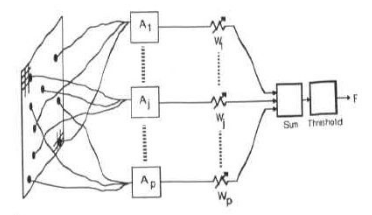
\includegraphics[width=0.5\textwidth]{perceptron.png}
\caption{Basic structure of a perceptron \cite{minsky1969perceptron}}
\label{fig:perceptron}
\end{figure}

Following Figure \ref{fig:perceptron}, we can see the perceptron receives \textit{p} inputs, $A_1$, $A_2$, ..., $A_p$ (or $x_1$, $x_2$, ..., $x_p$, depending on the source. 
The inputs are then respectively weighted by $w_1$, $w_2$, ..., $w_p$, which are real numbers indicating the importance of each of the input values. The output \textit{F} will then be calculated using the sum of those weighted inputs. 
Additionally, because the output is a binary value, a threshold is used to achieve the desired result. To be more specific, a perceptron is written as follows:

\begin{center}
$F = \begin{cases}
1 & if \sum_{i}^{p} A_i w_i \geq Threshold \\
0 & if \sum_{i}^{p} A_i w_i < Threshold
\end{cases}$
\end{center}

Consequently, the output of a perceptron is controlled by two things: the weights $w_1$, $w_2$, ..., $w_p$ and the Threshold. 
In modern neuron networks, however, the equation changed a bit by bringing the Threshold to the other side of the inequalities. 
The additive inverse of Threshold is then known as Bias, and the perception will be rewritten as:

\begin{center}
$F = \begin{cases}
1 & if \sum_{i}^{p} A_i w_i + Bias \geq 0 \\
0 & if \sum_{i}^{p} A_i w_i + Bias < 0
\end{cases}$
\end{center}

\subsubsection{Activation function}

Perceptron is the precursor to modern artificial neurons. Instead of returning only a binary output, an artificial neuron now produces values that are anywhere in the range [0,1]. 
The reason is to help in the learning process of a network. Neural networks can learn, i.e., finding the appropriate weights and biases given sufficient input data. 
The learning process, however, needs to be progressive, which means weights and biases get increasingly close to the "good" values. 
Having a binary output for each of the neurons makes it hard for this process to be done. 
For training a neural network, we use an error function to see how far or close the network is to the optimal results.
Because of the binary output of perception, a small change in the network's parameters can lead to a stark difference for the output, making it hard to tune the parameters to achieve a good result. 
Therefore, modifications must be made to the original perceptron model. 
Instead of using 0 as the threshold at which signals are allowed to be fired, we can use an activation function to map the output to the range we need appropriately.

\begin{figure}[htbp!] 
\centering    
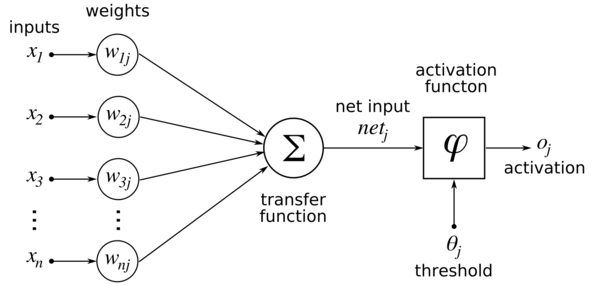
\includegraphics[width=0.7\textwidth]{artificial_neuron.png}
\caption{Structure of an artificial neuron \cite{wikian}}
\label{fig:artificial-neuron}
\end{figure}

The activation function takes as input the weighted sum of the input values fed to the perceptron and returns a value in the range [0,1]. 
Historically, the Sigmoid function was used for this purpose as it can squash the sum to the desired range \cite{li2015cs231n}. 
Modern networks, however, use different functions as well, such as hyperbolic tan function (tanh) or rectified linear unit (ReLU), to achieve better performance \cite{li2015cs231n}.

\subsubsection{Feedforward and Backpropagation}

Two operations are particularly important in neural networks: Feedforward and Backpropagation.

Feedforward is used in both the training and testing stage of a network. 
The task we need to do in feedforward is straightforward: Passing output of a layer as the input of the next layer.
Since all we are doing is unidirectionally putting values through the network from the input layer to the output layer, the operation is called feedforward. 

Backpropagation is generally used in the training stage to help neural networks learn their parameters, and it is considered an optimization. 
Different from feedforward, the job of this operation is to propagate error of the output values back to the network to update the network parameters. 
Backpropagation works by first do the normal feedforward operation on the network with the given input. 
After the output is obtained, we compare the output to the desired output, using a loss function to generate an error term for each of the neuron in the output layer. 
The error values are then propagated backward from the output layer until every neuron receive their respective error term. 
The error terms will be used to calculate the gradient, with which we can update the weights of the network to minimize the loss function as the process repeats. 
To find the most fitting parameters, gradient descend algorithm is usually applied.

\section{Classification Metrics}

In this section, we review how to use several common metrics that are used to evaluate predictions for classification problems.

\subsection{Logarithmic Loss}

Logarithmic loss, or log-loss for short, is a performance metric for evaluating the predictions of probabilities of membership to a given class.

Log-loss takes into account the uncertainty of your prediction based on how much it varies from the actual label, which gives us a more nuanced view of the performance of our model.
In binary classification, with $y$ is a binary indicator (0 or 1) of whether class label $c $is the correct classification and $p$ is the model predicted probability, the formula equals:

\bigskip
\begin{center}
    $LogLoss = -(y\log(p) + (1 - y)\log(1 - p))$
\end{center}
\bigskip

The scalar probability between 0 and 1 can be seen as a measure of confidence for a prediction by an algorithm.
Smaller log-loss is better with 0 representing a perfect log-loss.

\subsection{Confusion Matrix}
\label{ssec:confusion_matrix}

\begin{figure}[H]
    \centering    
    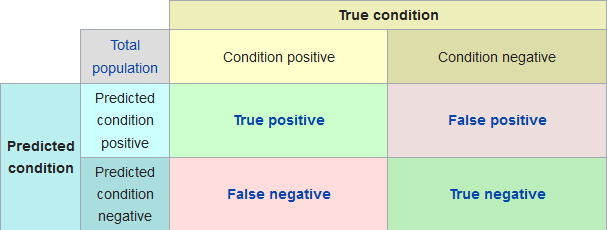
\includegraphics[width=0.7\textwidth]{confusion_matrix.png}
    \caption{Confusion matrix \cite{wiki_confusion_matrix}}
    \label{fig:confusion_matrix}
\end{figure}

A clean and unambiguous way to show the prediction results of a classifier is to use a confusion matrix (also called a contingency table).
For a binary classification problem, the table has two rows and two columns (which is shown in Figure \ref{fig:confusion_matrix}). 
Across the top is the actual class labels and down the side are the predicted class labels. 
Each cell carries the number of predictions made by the classifier that fall into that cell.

\begin{figure}[H]
    \centering    
    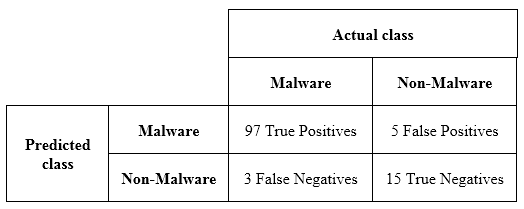
\includegraphics[width=0.7\textwidth]{confusion_matrix_example.png}
    \caption{An example of confusion matrix}
    \label{fig:confusion_matrix_example}
\end{figure}

Figure \ref{fig:confusion_matrix_example} is an example of binary classification in malware detection. 
Some of the input files are malware, and our test correctly says they are positive. 
They are called true positives (TP). 
In contrast, some are malware, but the test incorrectly claims they are not. 
They are called false negatives (FN). 
Some are clean files, and the test says they are not malware – true negatives (TN). 
Finally, there might be clean files have a positive test result – false positives (FP).

There are many derived ratios from confusion matrix, and the most common ones are listed below:

\begin{itemize}
    \item True Positive Rate (TPR), eqv. with hit rate, recall: $TPR = TP/P = TP/(TP + FN)$
    \item True Negative Rate (TNR): $SPC = TN/N = TN/(TP + FN)$
    \item Precision or Positive Predictive Value (PPV): $PPV = TP/(TP + FP)$
    \item Negative Predictive Value (NPV): $NPV = TN/(TN + FN)$
    \item Fall-out or False Positive Rate (FPR): $FPR = FP/N = FP/(TP + FN) = 1 - TNR$
    \item False Discovery Rate (FDR): $FDR = FN/(FN + TP) = 1 - PPV$
    \item Miss Rate or False Negative Rate (FNR): $FNR = FN/(FN + TP) = 1 - TPR$
\end{itemize}

\subsection{Overall Accuracy}

Overall accuracy is the number of correct predictions made as a ratio of all predictions made.

\begin{center}
    ${Accuracy} =  \cfrac{True\ positive + True\ negative}{Condition\ positive + Condition\ negative}$
\end{center}

Overall Accuracy essentially tells us out of all of the reference sites what proportion were mapped correctly. 
The overall accuracy is usually expressed as a percent, with 100\% accuracy being a perfect classification where all reference site were classified correctly. 
Overall accuracy is the easiest to calculate and understand but ultimately only provides the map user and producer with necessary accuracy information.

This is the most common evaluation metric for classification problems, it is also the most misused. 
It is only suitable when there is an equal number of observations in each class (which is rarely the case) and that all predictions and prediction errors are equally important (which is often not the case).

\subsection{Precision and Recall}

Precision can be thought of as a measure of a classifiers exactness. Precision attempts to answer the question "What proportion of positive identifications was actually correct?". A low precision can also indicate a large number of False Positives.

\begin{center}
    ${Precision} =  \cfrac{True\ positive}{True\ positive + False\ positive}$
\end{center}

Recall is the number of True Positives divided by the number of True Positives and the number of False Negatives. Computing in another way is the number of positive predictions divided by the number of positive class values in the test data. Recall attempts to answer "What proportion of actual positives was identified correctly?". It is also called Sensitivity or the True Positive Rate.

\begin{center}
    ${Recall} =  \cfrac{\sum True\ positive}{\sum Condition\ positive}$
\end{center}

\subsection{Area Under ROC curve}
\label{ssec:auroc}

Area Under the Receiver Operating Characteristic curve, AUROC or AUC for short, is a performance metric for binary classification problems. The AUROC has several equivalent interpretations:

\begin{itemize}
\item The expectation that a uniformly drawn random positive is ranked before a uniformly drawn random negative.
\item The expected proportion of positives ranked before a uniformly drawn random negative.
\item The expected true positive rate if the ranking is split just before a uniformly drawn random negative.
\item  The expected proportion of negatives ranked after a uniformly drawn random positive.
\item  The expected false positive rate if the ranking is split just after a uniformly drawn random positive.
\end{itemize}

An area of $1.0$ represents a model that made all predictions perfectly. A rough guide for classifying the accuracy of a classification test is the typical academic point system: 

\begin{itemize}
\item 0.9 - 1.0 = Excellent
\item 0.8 - 0.9 = Good
\item 0.7 - 0.8 = Fair
\item 0.6 - 0.7 = Poor
\item 0.5 - 0.6 = Fail
\end{itemize}

\subsubsection{Compute the AUROC}

Assume we have a binary classifier such as logistic regression. First, we compute two metrics from the confusion matrix (their formula are mentioned in section \ref{ssec:confusion_matrix}), which will be later combined into one:

\begin{enumerate}
    \item \textbf{True positive rate (TPR).} Intuitively this metric agrees to the proportion of positive data points that are correctly considered as positive, with respect to all positive data points. In other words, the higher TPR, the fewer positive data points we will miss.
    \item \textbf{False positive rate (FPR).} This metric corresponds to the proportion of negative data points that are mistakenly considered as positive, concerning all negative data points. In other words, the higher FPR, the more negative data points will be misclassified.
\end{enumerate}

\begin{figure}[H]
    \centering    
    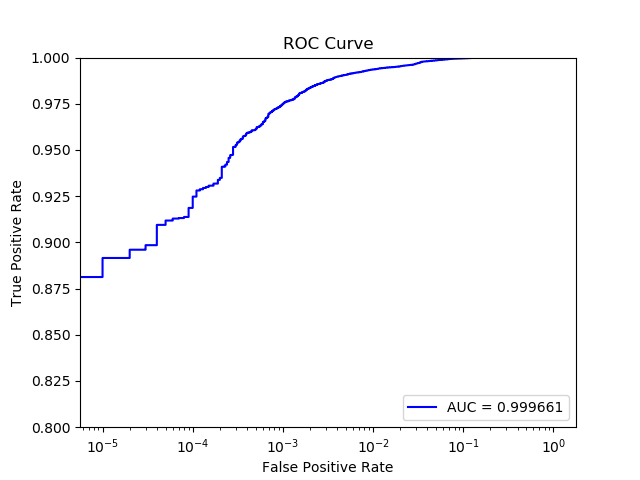
\includegraphics[width=0.8\textwidth]{roc_curve.png}
    \caption{An example of Receiver Operating Characteristic curve}
    \label{fig:auroc}
\end{figure}

Then, we combine the FPR and the TPR into one single metric by computing the two former metrics with many different threshold (for example, 0.00, $10^-5$, $10^-4$, $10^-3$, ..., 1.00, as shown as in Figure \ref{fig:auroc}) for the logistic regression, then plot them on a single graph, with the FPR values on the x-axis and the TPR values on the y-axis. The resulting curve is called  Receiver Operating Characteristic curve, and the metric we consider is the area under this curve.

\section{LightGBM - A Gradient Boosting Framework}

LightGBM, which means Light Gradient Boosting Machine, is a gradient boosting framework that uses tree-based learning algorithm \cite{ke2017lightgbm}. This framework is obtaining an extreme reputation due to its following advantages:

\begin{itemize}
\item Faster training speed and higher efficiency
\item Lower-memory usage
\item Better accuracy
\item Parallel and GPU learning supported
\item Capable of handling the large-scale data
\end{itemize}

The framework uses two following techniques to solve problems when the feature dimension is high, and data size is considerable: Gradient-based One-Side Sampling and Exclusive Feature Bundling.

\subsection{Gradient-based One-Side Sampling}

Base on the notice that, while there is no weight for data instance in the gradient-boosting decision tree, data instances with different gradients play different roles in the computation of information gain. 
In particular, according to the definition of information gain, instances with larger gradients (i.e., under-trained instances) will contribute more to the information gain.
Since, when subsampling the data instances, to retain the accuracy of information gain estimation, LightGBM tends to keep instances with large gradients (e.g., larger than a pre-defined threshold, or among the top percentiles), and only randomly drops instances with small gradients.
They proved that such a treatment could lead to a more accurate gain estimation than uniformly random sampling, with the same target sampling rate, especially when the value of information gain has a vast range.

\subsection{Exclusive Feature Bundling}

Regularly in real applications, although there are a large number of features, the feature space is quite sparse, which provides the LightGBM a possibility of using a nearly lossless approach to reduce the number of active features.
In fact, in a sparse feature space, many features are almost exclusive, i.e., they rarely take nonzero values together, e.g., the one-hot encoding features, therefore, the framework could safely bundle such unique features.
LightGBM uses an efficient algorithm named Exclusive Feature Bundling, which is a greedy algorithm with a constant approximation ratio.
Specifically, they reduce the optimal bundling problem to a graph coloring problem by taking features as vertices and add edges for every two features if they are not together exclusive.
